\begin{center}
                                \tablehead{\hspace{1cm}\\}
                                \tabletail{\hspace{1cm}\\}
                                \begin{supertabular}{p{0.5\textwidth}p{0.5\textwidth}}
                                \shrinkheight{1in}
                                \multicolumn{2}{p{\textwidth}}{The following bar chart shows how frequently various types of maintenance issue -- including compactor-related problems, pest problems, and plumbing issues -- occur in compactor locations consolidation-wide.} \\
                                \multicolumn{2}{c}{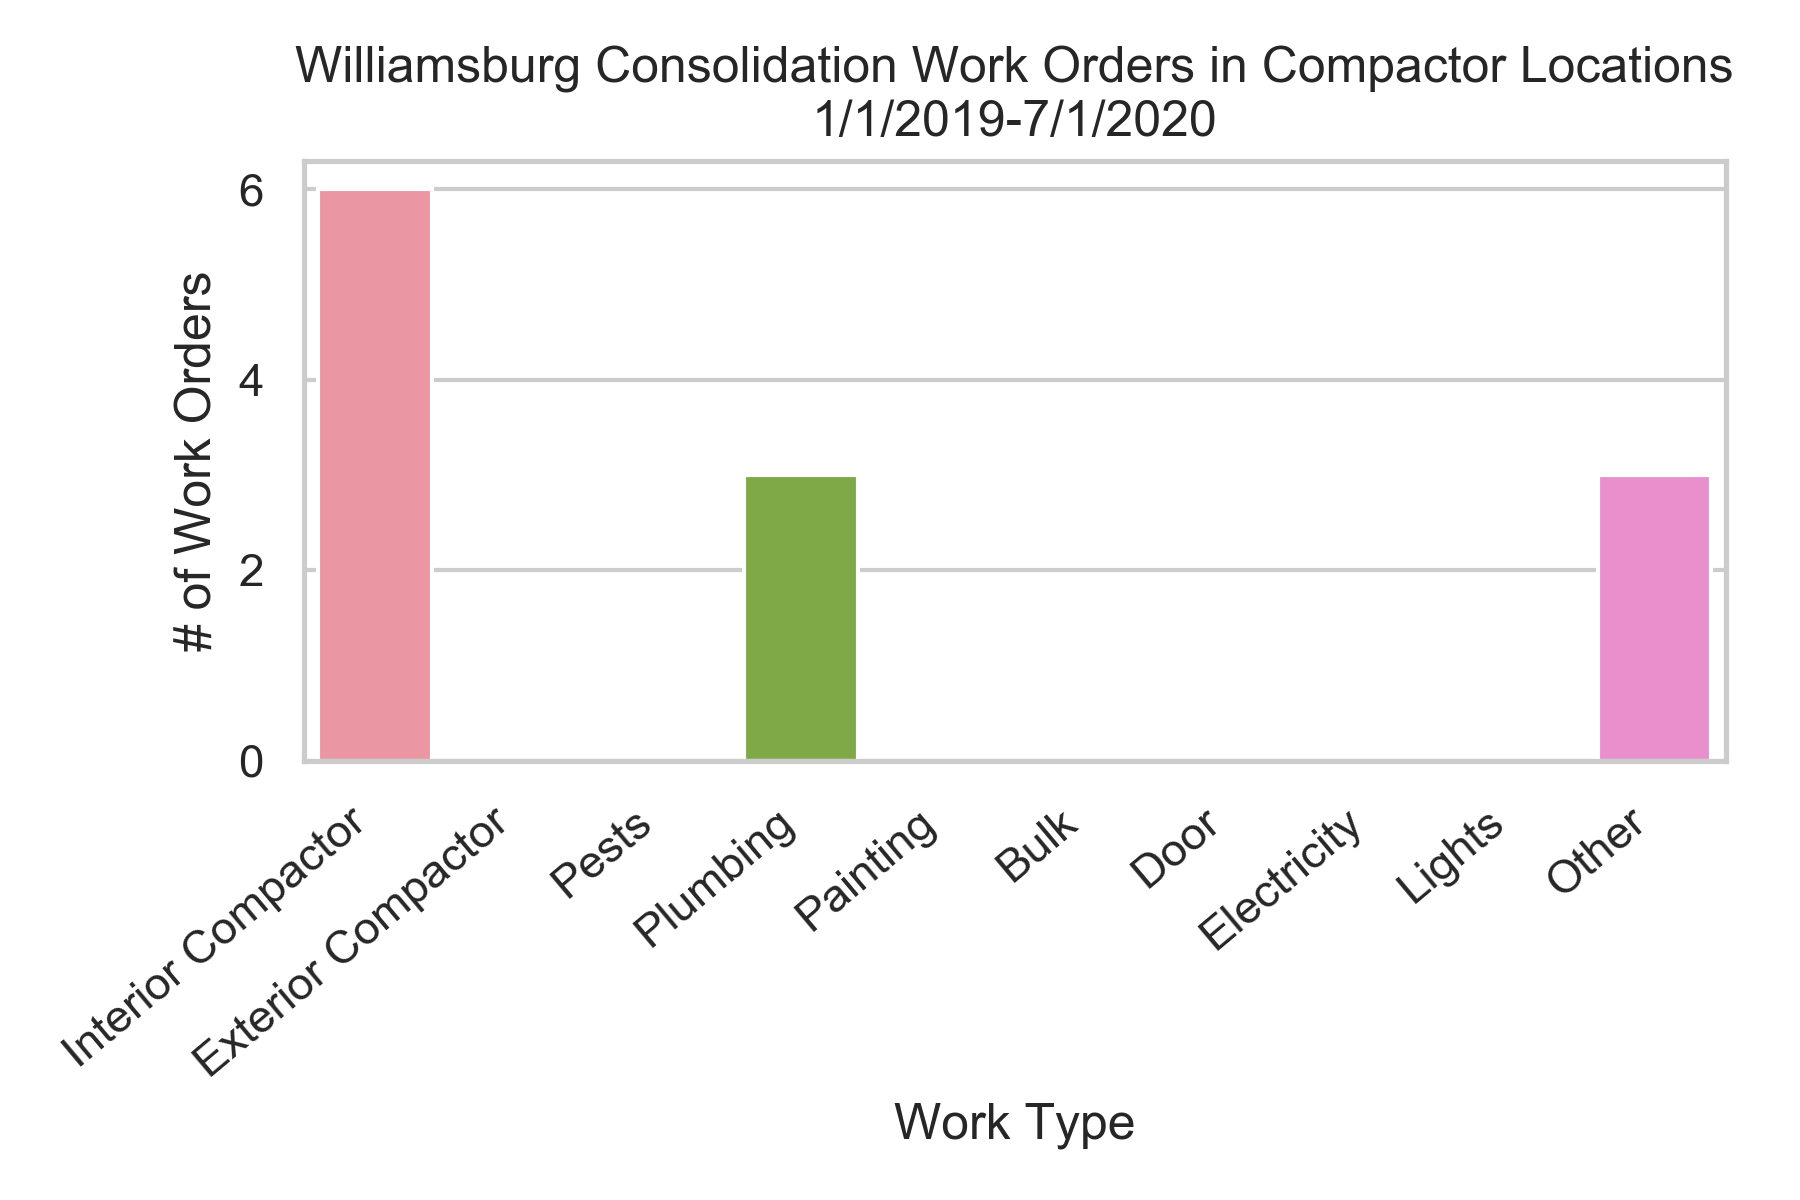
\includegraphics[width=0.6\textwidth]{\rootpath/WORK_ORDER_ANALYSIS/Consolidation_BarCharts/png/2_Williamsburg_WorkOrder_Category_BarChart.png}} \\
                                \end{supertabular}
\end{center}

                        \begin{center}
                        \tablehead{\hspace{1cm}\\}
                        \tabletail{\hspace{1cm}\\}
                        \begin{supertabular}{p{0.5\textwidth}p{0.5\textwidth}}
                        \multicolumn{2}{p{\textwidth}}{The following figures highlight repairs conducted in interior compactor locations at each major development, as well as within up to five buildings at each development.} \\
                        \multicolumn{2}{c}{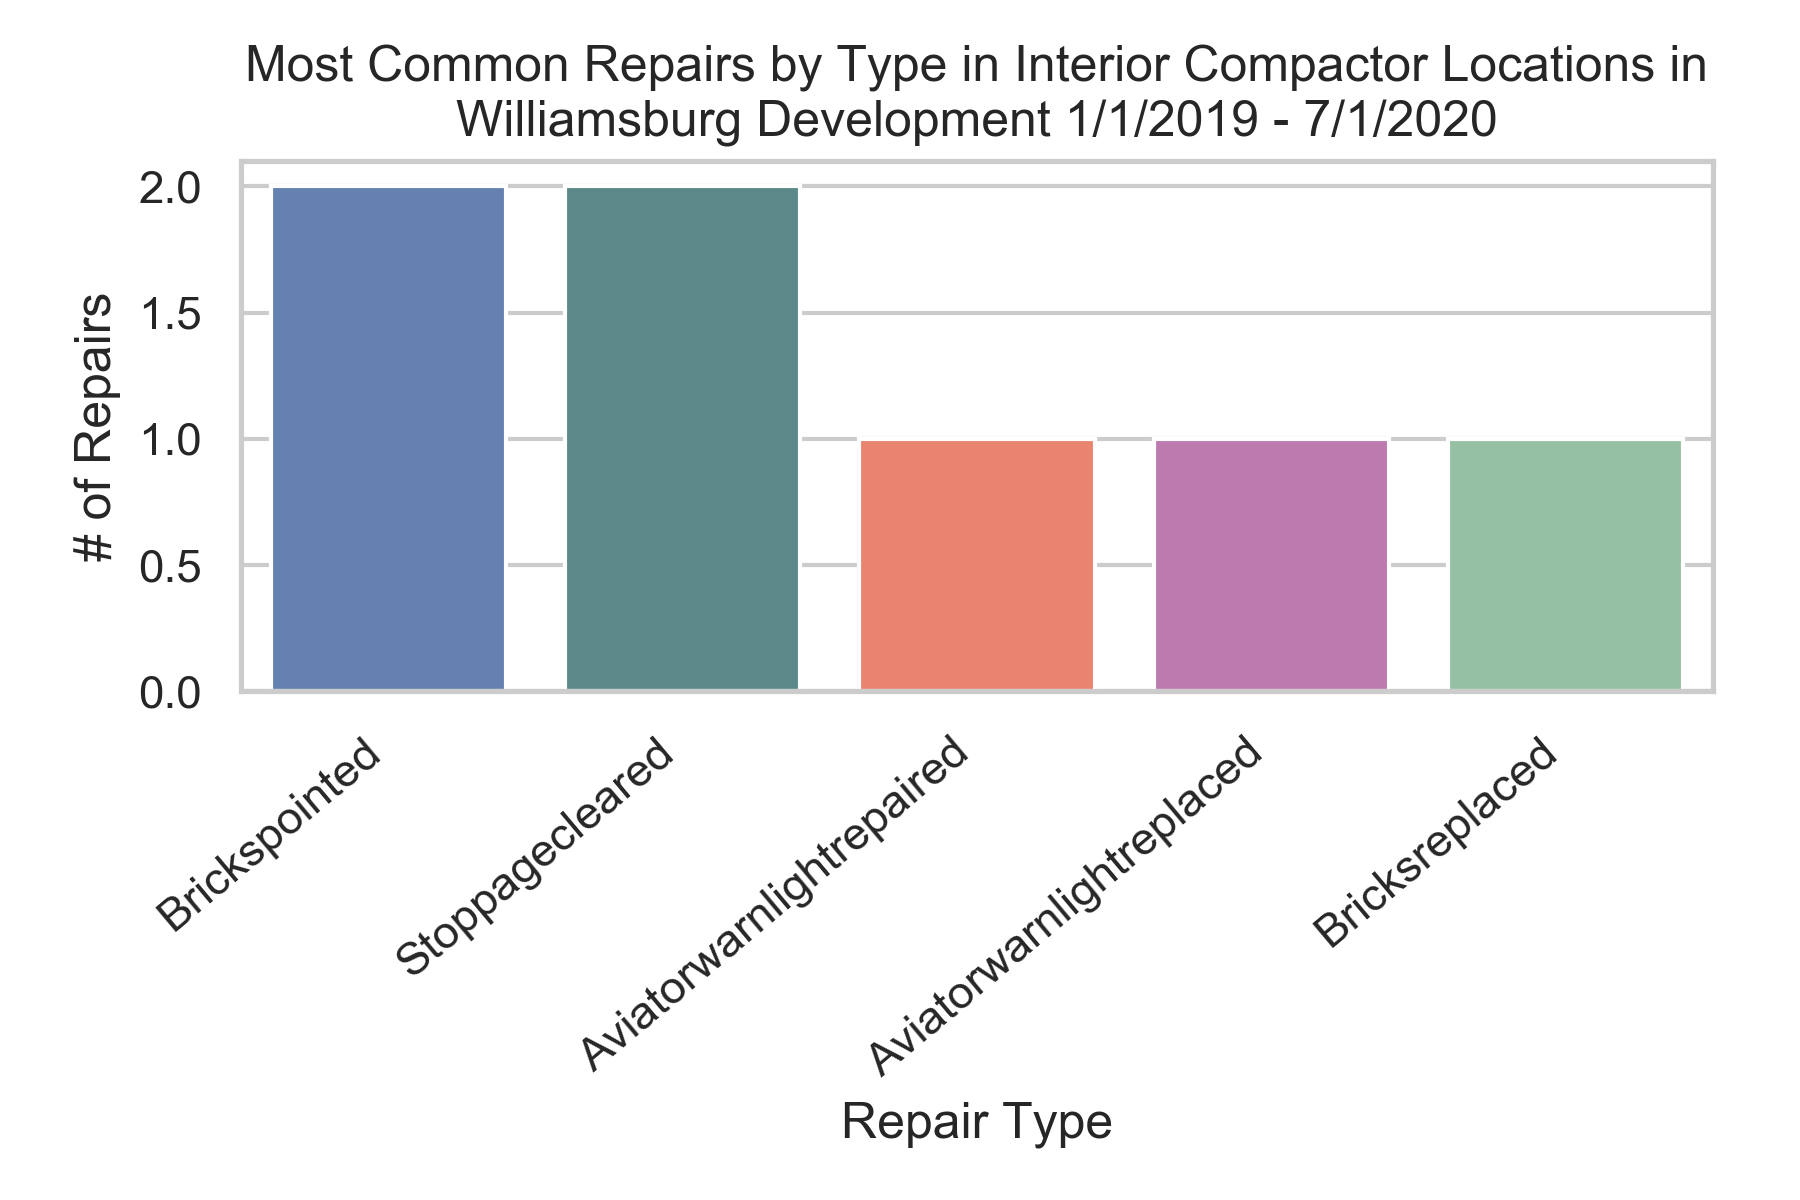
\includegraphics[width=0.6\textwidth]{\rootpath/WORK_ORDER_ANALYSIS/Dev_Interior_Comp_Repair_BarCharts/png/Williamsburg_2_Williamsburg_2_Interior_Comp_Rep_BarChart.png}} \\
                                    \multicolumn{2}{c}{\input{\rootpath/WORK_ORDER_ANALYSIS/Dev_Interior_Comp_Repair_Tables/\tds_repair_table}} \\
                                    \end{supertabular}
                                    \end{center}
                                    